\pagebreak

\section{Inferenz Statistik}

\subsection{Motivation}

In der Schließenden Statistik werden die Ergebnisse (Parameter der Grundgesamtheit) überprüft und zu verifizieren, ob die usprüngelichen Annahmen über das Statisches Experiment zu treffen und ob die Stichprobe ausreichend Informationen enthält, eine solche Aussage zu treffen.
 
Die Essenz ist daher, anhand einer bekannten Stichproben $x$ einen unbekannten Parameter $\varTheta$ zu schätzen. Dafür konstruiert man einen \textit{Schätzer}.\\

Im Folgenden wird der Schwerpunkt der Beispiele darauf liegen, dass es sich bei den \textit{Parametern der Grundgesamtheit} um Parameter des \gls{SM} handelt - der Verteilungsfunktion. Bei den Regressionparameter gelten in den meisten Fällen die gleichen Definitionen. Die Definitionen beschreiben im Kern, wie mit den Daten der Stichproben umgegangen werden soll. Eine Einschränkung auf Parameter der Verteilungsfunktion ist in der Regel nicht gegeben.

\subsection{Schätztheorie}
\subsubsection{Statistik}
\paragraph{Definition Statistik und Abgrenzung zum Schätzer}
\begin{Definition}{Statistik}
Sei $\left(\Omega, \SigmaAlgebra\right)$ ein \textit{messbarer Raum}\footnote{Hinweis zur Regression: Es wird hier nicht auf eine Wahrscheinlichkeitsraum verwiesen. Für die Abbildung werden nur die Werte aus $\Omega$ auf $\beta$ abgebildet. Für $\Omega$ kann auch gelten, dass es sich hierbei um einen Vektor handelt. So könnten verschiedenen Variablen $X$ und $Y$ auf einen andere Menge abgebildet werden.} und $\left(\beta, \SigmaAlgebraIndividuel{\beta}$  ein weitere \textit{messbarer Raum}, so heißt eine \textit{messbare Abbildung}\footnote{Siehe Definition Messbare Abbildung \refDefinition{Messbarkeitseigenschaft}}
\begin{align}
	S: \left(\Omega, \SigmaAlgebra\right) \rightarrow \left(\beta, \SigmaAlgebraIndividuel{\beta}
\end{align}
eine \textbf{Statistik}.
\end{Definition}

Eine \textit{Statistik} unterscheidet sich strukturell nicht von
\begin{itemize}
	\item von einer Schätzfunktion,
	\item einer Zufallsvariable (Abbildung),
	\item einem Punktschätzer oder
	\item einer messbaren Funktion (\refDefinition{Messbarkeitseigenschaft}).
\end{itemize}

Im Kern steht, dass mit dieser Konstruktion Verteilungen und Bildmaße ermöglichen.\\

Der Unterschied, zwischen \textit{Statistik} und \textit{Schätzfunktion}, liegt in der Verwendung und Interpretation\footnote{Bei der Schätzfunktion werden nicht binden, weitere Eigenschaften gefordert. Somit bleibt die Definition die gleiche.}

\begin{description}
	\item[Statistik] Ziel ist es Ordnung und Struktur aus den vorhanden Informationen (Daten) zu gewinnen. Dabei soll die Beobachtungstiefe reduziert werden. 
	\item[Schätzfunktion] Ziel ist hier mit den vorhanden Daten ($\left(\Omega, \SigmaAlgebra \right)$) eine Auswertung zu gewinnen, um unbekannte Parameter/ Werte bestmöglich zu \textit{schätzen}. Die Schätzfunktion unterliegt hier Gütekriterien.
\end{description}

\paragraph{Beispiele für Statistiken und Schätzfunktionen}
Wie schon oben mehrmals erwähnt, eine Statistik teilt sich den Aufbau mit der Schätzfunktion und weiteren Objekten. Das Ziel ist jedoch eine Struktur oder eine Beschreibung (Deskriptive Statistik) zu bewinnen.\\

\begin{itemize}
	\item Die \textbf{Ordnungsstatistik} gibt den $i$-ten kleinsten Wert einer Stichprobe an.\\
	\item Eine \textbf{Teststatistik}, auch \textit{\textbf{Prüfgröße}} oder \textit{\textbf{Testgröße}} genannt, wird als Hilfsfunktion in der mathematischen Statistik im Bereich der Testtheorie verwendet. Bei einem Hypothesentest wird die \textit{Nullhypothese} abgelehnt, wenn die \textit{Teststatistik} einen gewissen Wert $k$ über oder unterschreitet.
\end{itemize}


Am Beispiel der Tesstatistik: Gegeben sei 
\begin{align}
	T: \Stichprobenmenge \rightarrow \R,
\end{align} die \textit{Teststatistik}, sowie ein \textit{statistischer Test}
\begin{align}
	\phi: \Stichprobenmenge \rightarrow [0,1],
\end{align}
mit 
\begin{align}
	\phi(X) = \begin{cases}
		1 & \text{falls} T(X) > k,
		0 & \text{falls} T(X) <= k
	\end{cases}
\end{align}
hierbei ist $k$ eine feste Zahl, die auch kriterischer Wert genannt. Ist $T$ ein $z-$Statistik, 
\begin{align}
	\overline{X} = \frac{1}{n}\left(X_1 + X_2 + \dots, X_n\right)
\end{align}
das Stichprobenmittel, $\Stichprobenmenge = \R^n$, ist eine typische Teststatistik
\begin{align}
	T(X) =\sqrt{n} \frac{\overline{X} - \mu}{\sigma}
\end{align}
Die \textbf{Teststatistik} ist standardnormalverteilt mit $T\sim \Normalverteilung{0,1}$. Für den $t-$Test ist die $t-$Statistik $t-$verteilt mit $T\sim t_{n-1}$.\\

Sei $X=\Menge{0,1}^n, \SigmaAlgebra = \Potenzmenge (X)$ und $\left(P_\vartheta\right)_{\vartheta \in \Theta} \right)=\Menge{Ber(n, \vartheta)
| \vartheta \in \Theta}$ das \SM. Das \textit{Stichprobenmittel}, als Schätzfunktion für den Parameter $\vartheta$, ist gegeben durch das
\begin{align}
	\hat{\Theta}&: X \rightarrow [0,1]\Leerzeichen\text{mit}\Leerzeichen, \\
	&\hat{\Theta}(x) = \frac{1}{n}\sum_{i=1}^{n} x_i
\end{align}
\textit{Stichprobenmittel}. Eine Statistik könnte sein
\begin{align}
	M:X\rightarrow \R
\end{align}
mit $M(x)= \sum x_i$ als Statistik. Mit der Statistik $M$ wird nicht der Parameter $\vartheta = p$ geschätzt, sondern nur eine Informationsreduktion vorgenommen.\footnote{
	Quelle: \href{Statistik (Funktion)}{https://de.wikipedia.org/wiki/Statistik_(Funktion)}, \href{Ordnungsstatistik}{https://de.wikipedia.org/wiki/Ordnungsstatistik}
}

\subsubsection{Schätzer}
\paragraph{Definition Schäter}
Wie erwähnt, ein \textit{Schätzer} oder auch \textit{Schätzfunktion} oder \textit{Schätzstatistik} genannt, ist eine Funktion aus den Daten der Stichproben eine Aussage über unbekannte Parameter einer Grundgesamtheit zu tätigen.\\

\begin{Lemma-Definition}{Stichprobenraum}
% Stichprobenraum Geschwunges X \mathcal{X}
Ein \textit{Stichprobenraum} $\mathcal{X}_n$ besteht aus der Menge aller möglichen Stichprobenwerte $\left(x_1, \dots, x_n\right)\in X_n \subseteq \R^n$.
\end{Lemma-Definition}

\begin{Definition}{Schätzer/Schätzfunktion}
Sei $\Psi$ eine Statistik auf $\left(\Omega, \SigmaAlgebra\right)$ nach $\left(\beta, \SigmaAlgebraIndividuel{\beta}$ (\refDefinition{Statistik}) und $X_1,\dots, X_n$ eine Stichprobe mit $(X_1,\dots,X_n)\in \Omega$. \\
Eine \textbf{Schätzer} für den Parameter $\vartheta$ oder den Funktionswert $\gamma$ ist eine Abbildung 
\begin{align}
	\Psi: \Omega \rightarrow \beta.
\end{align}
die messbar von $X_1,\dots,X_n$ abhängt.
\end{Definition}

Bei dem Schätzer\footnote{\href{Schätzfunktion}{https://de.wikipedia.org/wiki/Schätzfunktion}} sind drei Punkte besonders wichtig
\begin{itemize}
	\item Zu schätzen kann ein Wert $\vartheta$ oder eine Parameterfunktion/Kenngröße $\gamma$ sein.
	\item Ein Schätzer ist auch eine Zufallsvariable $\hat{\Theta}_n$ .
	\item Im Theoretischen wird mit den Zufallsvariablen $X_1,\dots,X_n$ im praktischen mit den Bildern der Zufallsvariablen/Stichprobenwerte $x_1,\dots,x_n$ gearbeitet.
\end{itemize}

\paragraph{Parameter oder Parameterfunktion}
In Verknüpfung mit der Entscheidungstheorie wird der Parameter nicht als Skalar abgebildet, sondern per Funktion, welche aus dem Parameterraum $\Theta$ in den Entscheidungsraum $\beta$ abbildet.
\begin{align}
	\gamma: \Theta \rightarrow \beta
\end{align}
Der Raum $\left(\beta, \SigmaAlgebraIndividuel{\beta}$ wird auch \textit{Entscheidungsraum} genannt. \footnote{\href{Parameterfunktion}{https://de.wikipedia.org/wiki/Parameterfunktion_(Statistik)}}.

Um genau zu sein, bildet die Entscheidungsfunktion in einen \textit{Entscheidungsraum} $(\beta, \SigmaAlgebraIndividuel{\beta}$.
\begin{Lemma-Definition}{Entscheidungsraum}
	Ein \textit{Entscheidungsraum} ist ein Messraum, bei dem die $\sigma-$Algebra alle einelementigen Mengen enthält, sodass $\forall \omega\in \Omega $ die Menge $\Menge{\omega} \in \SigmaAlgebraIndividuel{\beta}$ liegt. Beispielsweise ist $(\R, \SigmaAlgebraIndividuel{\R}$ ein Entscheidungsraum.
\end{Lemma-Definition}

\paragraph{Beispiel Parameterfunktion}
Für den Verteilungsparameter eine Bernoulli Verteilung $\vartheta$, wird dieser in der Regel mit dem Stichprobenmittel auf 
\begin{align}
	\gamma(\vartheta)=\vartheta
\end{align}
abgebildet.

Für die Normalverteilung wird für den Parameter $\sigma$ das Stichprobenmittel
auf 
\begin{align}
	\gamma(\sigma)=\sigma^2
\end{align}
abgebildet.

\paragraph{Symmetrie Schätzer als Zufallsvariable}

Wie in der Übersicht geschildert, wird aus der Schätzfunktion auch gleichzeitig eine eigene Zufallsvariable, siehe \ref{subsec_Dualitaet_DreiFaltigkeit}.

Die Abbildung $\Psi$ als Schätzer des Parameters $\vartheta$ ist gleichzeitig eine Zufallsvariable:

\begin{align}
	\hat{\Theta_n} := \Psi(X_1, \dots, X_n)
\end{align}
mit eigener Verteilung.

\begin{figure}[H]
	\centering
	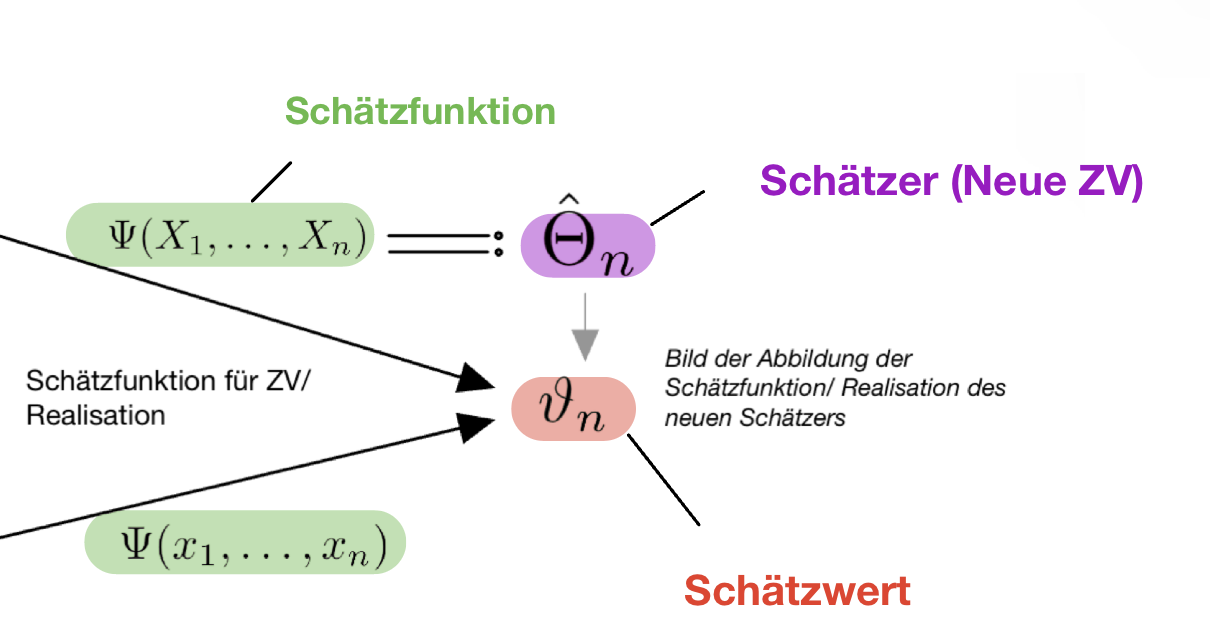
\includegraphics[width=0.7\linewidth]{attachment/chapter_13/Scc073}
	\caption{Drei Faltigkeit - Schätzer, Schätzfunktion und Schätzwert}
\end{figure}

Ebenso ist nochmals daraufhinzuweisen, dass es eine Unterschied zwischen der Funktion des Schätzers und des tatsächlichen Schätzwertes gibt.

\begin{figure}[H]
	\centering
	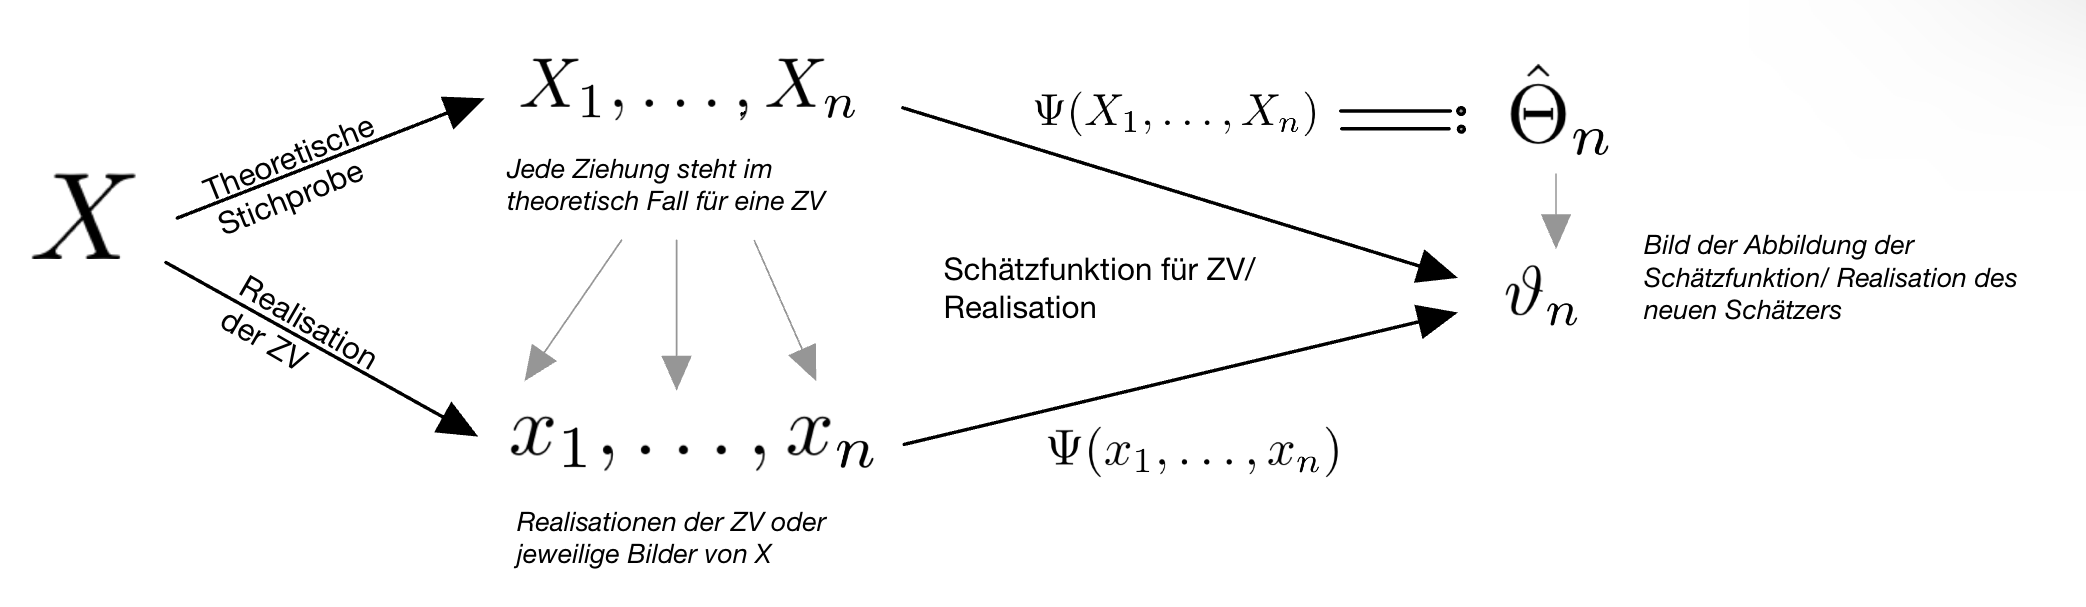
\includegraphics[width=0.7\linewidth]{attachment/chapter_13/Scc072}
	\caption{Theoretische und reale Betrachtung einer Stichprobe}
\end{figure}

Die Realisation von $\hat{\Theta}_n$ wird ebenfalls mit einem Dach versehen: $\hat{\vartheta}_n$

\paragraph{Verteilung der Schätzfunktion}
Wie im vorherigen Abschnitt erwähnt, ist die Schätzfunktion ebenso eine eigenen Zufallsvariaben $\hat{\Theta}$. Je nach Schätzfunktion besitzt diese eine eigene Verteilung. \\

Sei $X_1,\dots, X_n$ \gls{iid} Normalverteilt gilt für die Schätzfunktion, Stichprobenmittel
\begin{align}
	\hat{\Theta}\sim \Normalverteilung{\mu_X, \sigma_X/n}
\end{align}
Die Varianzschätzung $S_n^2$ um konstante Terme angepasst, verteilt sich wie folgt:
\begin{align}
	\frac{(n-1)S_n^2}{\sigma^2}\sim \mathbb{X}(n-1)
\end{align}
\footnote{Quelle: \href{Schätzfunktion, Wiki}{https://de.wikipedia.org/wiki/Schätzfunktion#Verteilung_der_Schätzfunktionen}}
\subsubsection{Eigenschaften von Schätzern}
In der klassischen Inferenz Statistik sind
\begin{itemize}
	\item Erwartungstreue/ Mediantreue
	\item Effizienz
	\item Konsitenz,
	\item Suffizienz
	\item Normalität
	\item Linearität
	\item Robustheit
\end{itemize}
die wichtigsten Eigenschaften eines Schätzer $\hat{\Theta}_n$. Einige der Eigenschaften sind asymptotisch: Verhalten von $\hat{\Theta}_n$ für $n\rightarrow \infty$.

\paragraph{Erwartungs- und Mediantreue}
\begin{Definition}{Erwartungstreue}
	Ein Schätzer $\hat{\Theta}_n$ heißt \textit{erwartungstreu} oder \textit{unverzerrt}, wenn 
	\begin{align}
		\Erwartungswert{\hat{\Theta}_n} = \gamma(\vartheta) \Leerzeichen \forall \vartheta \in \Theta.
	\end{align}
	oder simpler $\Erwartungswert{\hat{\Theta}_n} = \vartheta \Leerzeichen \forall$.
\end{Definition}
Für den Erwartungswert gilt wie unter \ref{paragraph: Erwartungswert}: 
\begin{align}
	 \Erwartungswert{\hat{\Theta}_n} := \int \hat{\vartheta}d P_{\hat{\Theta}_n}(\hat{\vartheta}_n)
\end{align}
Wiederholter Hinweis: Diese Eigenschaft ist \underline{nur} wichtig, dass die Eigenschaft erfüllt ist!\\

% Beispiel kommt aus dem Taschenbuch auf Seite 445
\textbf{Plausible Eigenschaft} Sei $\hat{\Theta}_n = \overline{X}_n = \frac{1}{n}\sum_i^nX_i$ das \textit{Stichprobenmittel} und $\vartheta = \Erwartungswert{X} = \mu$ mit $X_i \sim i.i.d.$ gilt
\begin{align}
	\Erwartungswert{\hat{\Theta}_n} &= 	\Erwartungswert{\overline{X}_n} \\
	&= 	\Erwartungswert{\frac{1}{n}\sum_i^nX_i}} \\
	&= \frac{1}{n}\sum_i^n \Erwartungswert{X_i} \\
	&= \frac{1}{n}n \mu \Leerzeichen \text{mit}\Leerzeichen \Erwartungswert{X_i}=\mu_i = \mu \\
	&= \mu 
\end{align}
Der Schätzer $\overline{X}_n$ ist erwartungstreu. Wäre $\gamma(\mu)=\mu$, wäre der Schätzer ebenso erwartungstreu.

Bezüglich der Verteilung von $\overline{X}_n$ ist gegeben durch $X_i\sim \Normalverteilung{\mu, \sigma^2}$\footnote{Jede Zufallsvariable steht in dem Fall für das gleiche Merkmal. In Stichproben können jedoch auch mehrere Merkmale betrachtet werden.} $\overline{X}_n\sim\Normalverteilung{\mu, \sigma^2/n}$.\\

\textbf{Erwartungstreu, aber riskant} Sei der Schätzer
\begin{align}
	\Psi(X_1,\dots, X_n)\mapsto X_1,
\end{align}
so ist der Schätzer erwartungstreu für $\mu$. Dies ist jedoch ein unplausibler Schätzer, weil nur die erste Beobachtung berücksichtigt wird.\\

Abschluss: Es gibt viele \textit{erwartungstreue} Schätzer die unplausible sind. Ein \textit{idealer} Schätzer ist ein solcher welcher für $\forall \vartheta \in \Theta$ und $(x_1,\dots,x_n)$ den wahren Wert für $\gamma(\vartheta)$ schätzt.

\paragraph{Konsitenz}
Bei der \textit{Konsitenz} geht es darum, dass mit einer höhere Stichprobe, die Abweichung, zwischen den Schätzerwert und den Parameter gegen null geht.

\begin{Definition}{Erwartungstreue}
	Sei $\Psi(X_1,\dots, X_n)$ eine \textit{Schätzer} für die Funktion $\gamma(\vartheta)$ für alle $\vartheta\in \Theta$. Für den unbekannten Parameter $\vartheta$ der Grundgesamtheit heißt $\Psi$ für ein beliebiges $\epsilon >0$ \textit{\textbf{konsitenz}}, wenn
\begin{align}
	\lim_{n\rightarrow \infty} P_{\vartheta}\left(\lvert \Psi(X_1,\dots,X_n) - \gamma(\vartheta)\rvert>= \epsilon \right) = 0
\end{align}	  
\end{Definition}
Mit zunehmenden $n$ wird die Wahrscheinlichkeitsdichte des Parameters $\gamma(\vartheta)$ schmaler. Somit wird für jedes höhere $n$ mehr Fläche zwischen $\Psi \pm \epsilon$ liegen.
\begin{figure}[H]
	\centering
	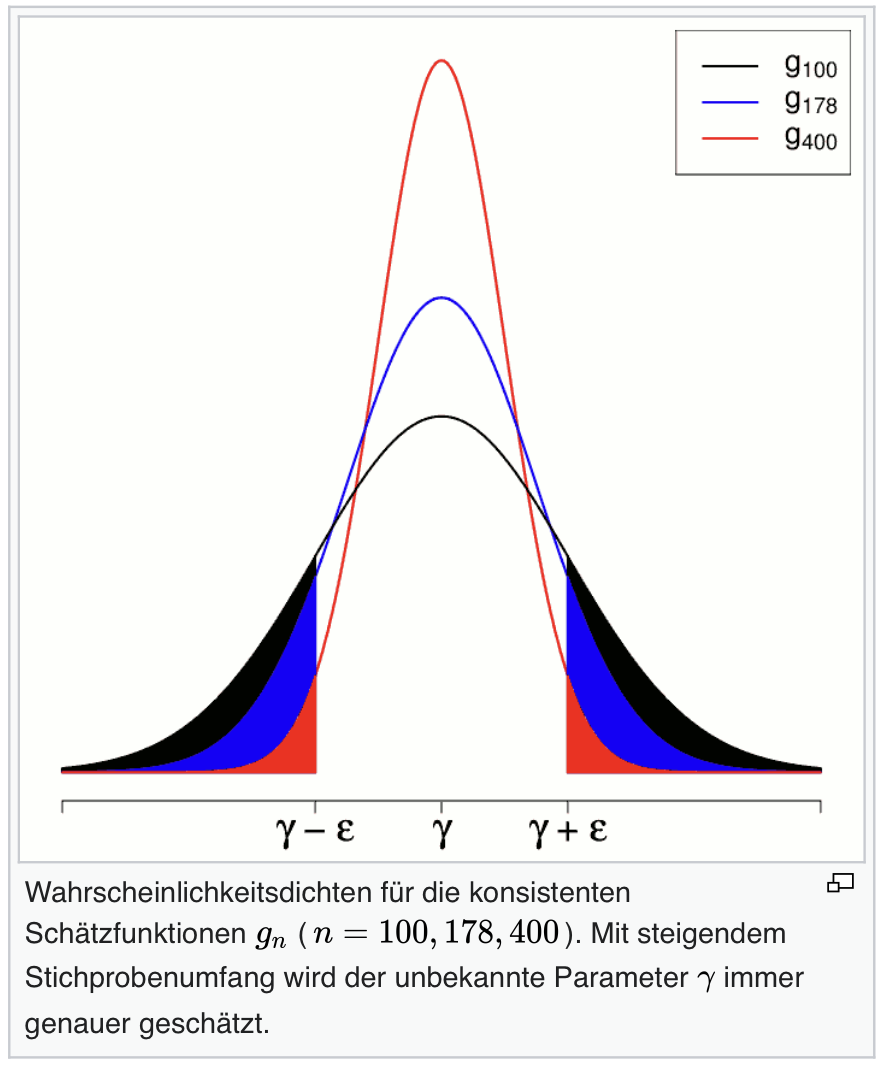
\includegraphics[width=0.7\linewidth]{attachment/chapter_13/Scc074}
	\caption{Wahrscheinlichkeitsdichte wird konzentierter um $\gamma$}
\end{figure}

\paragraph{Mittlere Quadratische Fehler (MSE)}
Die \gls{MSE} ist die Eigenschaft, welche untersucht, ob eine systematische Verzehrung vorliegt - ein Bias.

\begin{Definition}{Mittler Quadratischer Fehler (MSE)}
		Sei $\Psi(X_1,\dots, X_n)$ eine \textit{Schätzer} für die Funktion $\gamma(\vartheta)$ für alle $\vartheta\in \Theta$. Der \gls{MSE} definiert sich über 
\begin{align}
	MSE(\Psi, \gamma(\vartheta)):= \Erwartungswert{\lvert \Psi(X_1,\dots, X_n) -\gamma(\vartheta)\rvert^2} = \Varianz{\Psi} - Bias(\Psi)^2 , \vartheta\in \Theta  
\end{align}
\end{Definition}

Der Bias einer Zufallsvariablen definiert sich wie folgt:

\begin{Lemma-Definition}{Bias}
Sei $\Psi$ ein Schätzer für $\vartheta\in \Theta$:
	\begin{align}
		Bias(\Psi):= Bias(\Psi, \vartheta):= \Erwartungswert{\Psi} - \vartheta
	\end{align}
\end{Lemma-Definition}

\textbf{Herleitung des Mittleren Quadratischen Fehlers}\\

Durch gleichzeitige Addition und Subtration von $\Erwartungswert{\Psi}$ bleibt das Ergebnis unverändert:
\begin{align}
	MSE(\Psi) 
	&= \Erwartungswert{
		\left(
			\Psi(X_1,\dots, X_n) - \gamma(\vartheta)
		\right)^2
	} \\
	&= \Erwartungswert{
		\left(
			\Psi(X_1,\dots, X_n) 
			- \Erwartungswert{\Psi} + \Erwartungswert{\Psi} 
			- \gamma(\vartheta)
		\right)^2
	}  \Leerzeichen \text{mit}\Leerzeichen \Psi =  \Psi(X_1,\dots, X_n) \Leerzeichen \text{und}\Leerzeichen \gamma = \gamma(\vartheta)\\
	&= \Erwartungswert{
		\left(\Psi - \Erwartungswert{\Psi}\right)^2 
		+ 
		2\left(\Psi - \Erwartungswert{\Psi}\right)
		\left(\Erwartungswert{\Psi} - \vartheta \right) 
		- 
		\left(\Erwartungswert{\Psi} - \gamma \right)
	}\\
	&= \Erwartungswert{
		\left(\Psi - \Erwartungswert{\Psi}\right)^2 
		+ 
		2\left(\Psi - \Erwartungswert{\Psi}\right)
		\left(\Erwartungswert{\Psi} - \vartheta \right) 
		- 
		\left(\Erwartungswert{\Psi} - \gamma \right)^2
	}\\
\end{align}
Die Erwartungswert-Zerlegung erlaubt, dass der Erwartungswert auf die einzelnen additiven Teile angewandt werden kann.

\begin{align}
	\Erwartungswert{
		\left(\Psi - \Erwartungswert{\Psi}\right)^2
	}
	+
	\Erwartungswert{ 
		2\left(\Psi - \Erwartungswert{\Psi}\right)
		\left(\Erwartungswert{\Psi} - \vartheta \right) 
	}
	-
	\Erwartungswert{ 
		\left(\Erwartungswert{\Psi} - \gamma \right)^2
	}
\end{align}
Der Mittlere Termin mit $\Erwartungswert{\Psi} - \Erwartungswert{\Psi}$ wird zu Null. Der letzte Teil wir zu
\begin{align}
	\Erwartungswert{\left(\Erwartungswert{\Psi} - \gamma \right)^2} &=
	\Erwartungswert{
		\left(\Erwartungswert{\Psi} - \gamma \right)
		\left(\Erwartungswert{\Psi} - \gamma \right)
	}\\
	&= \left(\Erwartungswert{\Psi} - \gamma \right)^2\\
	&= Bias(\Psi)^2
\end{align}
Der erste Termin ist die Varianz, was zum Schluss ergibt:
\begin{align}
	MSE(\Psi) & = 	\Varianz{\Psi} - Bias(\Psi)^2
\end{align}
\footnote{Quellen hierfür sind: \href{Uni Berlin}{https://wikis.hu-berlin.de/mmstat/Mittlere_quadratische_Abweichung_(stochastisch)}, \href{Schätzfunktion}{https://de.wikipedia.org/wiki/Schätzfunktion#Konsistenz}}

\subsubsection{Methoden zur Schätzfunktionen Konstruktion}
% Quelle: https://www.uni-ulm.de/fileadmin/website_uni_ulm/mawi.inst.110/lehre/ss13/Stochastik_I/Skript_5.pdf

In Folgenden werden Methode,
\begin{itemize}
	\item Momentummethode,
	\item Maximum-Likelihood Methode,
	\item Kleinstes Quadrate Methode,
	\item Bayer Methode
\end{itemize}
aufgezeigt, mit welche Schätzfunktionen konstruiert werden. Im Abschnitt zuerst wurde aufgezeigt, welche Eigenschaften eine Schätzer bewerten.


\paragraph{Momenten Methode}
Am Beispiel der Normalverteilung werde die Parameter $\mu$ und $\sigma$. 